\documentclass[11pt,a4paper]{article}
\usepackage[utf8]{inputenc}
\usepackage[T1]{fontenc}
\usepackage{array}
\usepackage{amsmath}
\usepackage{amsfonts}
\usepackage{siunitx}
\usepackage{placeins}
\usepackage{amssymb}
\usepackage{makeidx}
\usepackage{sidecap}
\usepackage{fvextra}
\usepackage{multicol}
\usepackage{listings}
\usepackage{appendix}
\usepackage{comment}
\usepackage{nicematrix}
\usepackage{multirow}
\usepackage{braket}
\usepackage{graphicx}
\usepackage{relsize}
\usepackage{fancyhdr}
\usepackage{cprotect}
\usepackage{color} 
\usepackage{hyperref}
\hypersetup{
	colorlinks=true, 
	linktoc=all, 
	linkcolor=blue,
	urlcolor=blue
}
\usepackage[left=2cm,right=2cm,top=1.5cm,bottom=2cm]{geometry}
\usepackage{titling}
\usepackage{etoolbox}
\flushbottom
\title{Statistical Analysis of Experimental Data\\
	\vspace{0.2cm}
	\large{Homework 02}}
\vspace{-0.2cm}
\author{Igor Di Tota}
\date{\small \url{https://github.com/igordt/SAED_homeworks/tree/main}}


\begin{document}
	\maketitle
	
	\section*{Introduction}
	
	This homework concerns the Bertrand paradox: \textit{in a circle of radius $R$ an equilateral triangle is drawn.
	What is the probability that a random chord is longer than the side of the triangle?}\\
	
	As demonstrated in the lecture, the answer depends on how a random chord is defined.
	Below, I present my own definition of a random chord, the distribution of chords generated using this method, and the resulting probability.
	
	\section*{Definition of the random chord}
	
	A random chord is generated as follows:
	\begin{enumerate}
		\item two points $P_1$ and $P_2$ are chosen independently and uniformly distributed inside the disk of radius $R$;
		\item the chord is the segment of the line through $P_1$ and $P_2$ delimited by the circle.
	\end{enumerate}
	Whether the circumference belongs to the set of possible points or not does not matter: it has zero area, so the probability that a point lies exactly on it is zero.
	
	\subsection*{Uniform points inside the disk}
	
	\emph{Uniformly distributed inside the disk} means that the probability of finding a point in a region is proportional to its area.
	In polar coordinates $(r, \varphi)$ the angle $\varphi$ can be taken uniform in $[0, 2\pi)$.
	For the radius, the first naive choice would be $r = R\,U$, with $U$ uniform in $[0, 1)$.
	With this choice every ring of equal thickness $dr$ receives the same number of points, but the area of a thin ring between $r$ and $r + dr$ is
	\begin{equation}
		dA = 2\pi r\, dr,
	\end{equation}
	which grows with $r$. The density of points per unit area would then be
	\begin{equation}
		\frac{dN}{dA} \propto \frac{dr}{2\pi r\, dr} \propto \frac{1}{r},
	\end{equation}
	so the points would accumulate near the centre.
	
	To have points uniform in area, the probability of being in a ring must be proportional to its area.
	The probability density of $r$ and its cumulative distribution\footnote{The cumulative distribution function $F_X(x)$ of a random variable $X$ is the function that gives the probability that $X$ takes a value less than or equal to a specified value $x$.} are therefore
	\begin{equation}
		f(r) = \frac{2r}{R^2}, \qquad F(r) = \int_0^r f(r')\, dr' = \frac{r^2}{R^2}, \qquad 0 \le r \le R .
	\end{equation}
	Using the inverse transformation:
	\begin{equation}
		U = F(r) = \frac{r^2}{R^2} \quad \Longrightarrow \quad r = R\sqrt{U}.
		\label{eq:sqrt}
	\end{equation}
	
	\subsection*{Chord from the two points}
	
	The line through $P_1 = (x_1, y_1)$ and $P_2 = (x_2, y_2)$ is written in parametric form as
	\begin{equation}
		x(t) = x_1 + t\,\Delta x, \qquad y(t) = y_1 + t\,\Delta y, \qquad \Delta x = x_2 - x_1, \quad \Delta y = y_2 - y_1 .
	\end{equation}
	Imposing $x(t)^2 + y(t)^2 = R^2$ gives the second-degree equation
	\begin{equation}
		a\,t^2 + b\,t + c = 0, \qquad a = \Delta x^2 + \Delta y^2, \quad b = 2(x_1\Delta x + y_1\Delta y), \quad c = x_1^2 + y_1^2 - R^2 .
	\end{equation}
	Since $P_1$ is inside the circle, $c \le 0$ and the discriminant $b^2 - 4ac$ is always non-negative.
	The two solutions $t_\pm$ give the endpoints $A$ and $B$ of the chord, and its length is $L = |B - A|$.
	
	The procedure is illustrated in Figure~\ref{fig:definition}.
	
	\begin{figure}[!h]
		\centering
		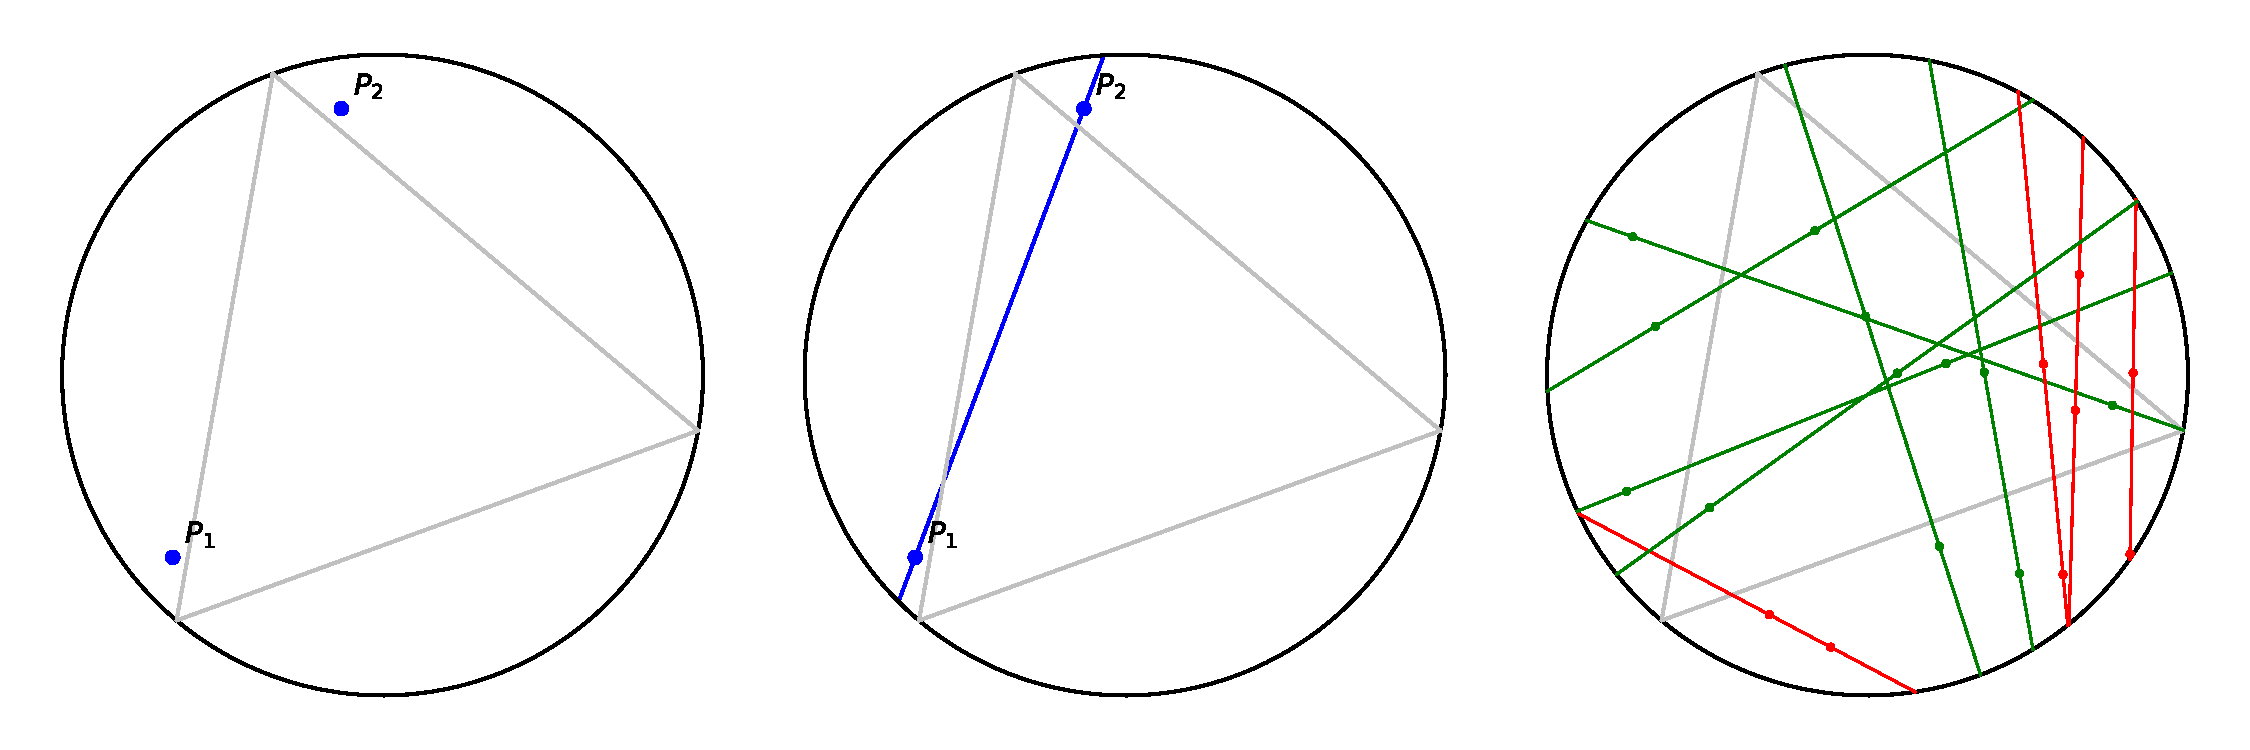
\includegraphics[width=\linewidth]{images/chord_definition.pdf}
		\caption{Definition of the random chord. Left: two random points $P_1$ and $P_2$ uniformly distributed inside the disk. Centre: the chord through the two points. Right: ten examples of random chords with their generating points; the chord is green if it is longer than the side of the inscribed triangle, red otherwise.}
		\label{fig:definition}
	\end{figure}
	\FloatBarrier
	
	\section*{Distribution of the chords and probability}
	
	Following the procedure described above, $N = 1000$ random chords are generated.
	For each chord the length $L$ is compared with the side of the triangle $\ell = R\sqrt{3}$, and the probability is estimated as the fraction of chords longer than the side:
	\begin{equation}
		P = \frac{n_{long}}{N}.
	\end{equation}
	
	Each chord is an independent Bernoulli trial (two possible outcomes: longer or shorter than the side), so $n_{long}$ follows a binomial distribution with variance $\mathrm{Var}(n_{long}) = N P (1 - P)$.
	The uncertainty on the fraction $P = n_{long}/N$ is then\footnote{For a random variable $X$ and a constant $a$, $\mathrm{Var}(aX) = a^2\,\mathrm{Var}(X)$.
		With $X = n_{long}$ and $a = 1/N$ this gives $\mathrm{Var}(P) = \mathrm{Var}(n_{long})/N^2 = P(1-P)/N$.
	}
	\begin{equation}
		\sigma_P = \sqrt{\frac{\mathrm{Var}(n_{long})}{N^2}} = \sqrt{\frac{P(1-P)}{N}} .
		\label{eq:sigma}
	\end{equation}
	
	Out of $N = 1000$ chords, $n_{long} = 736$ are longer than the side of the triangle, which gives
	\begin{equation}
		P = 0.736 \pm 0.014 .
	\end{equation}
	
	The generated chords are shown in Figure~\ref{fig:distribution}.
	The chords cross the central region of the disk more often, and most of them are longer than the side of the triangle; the shorter chords are found near the border of the circle.
	
	\begin{figure}[!h]
		\centering
		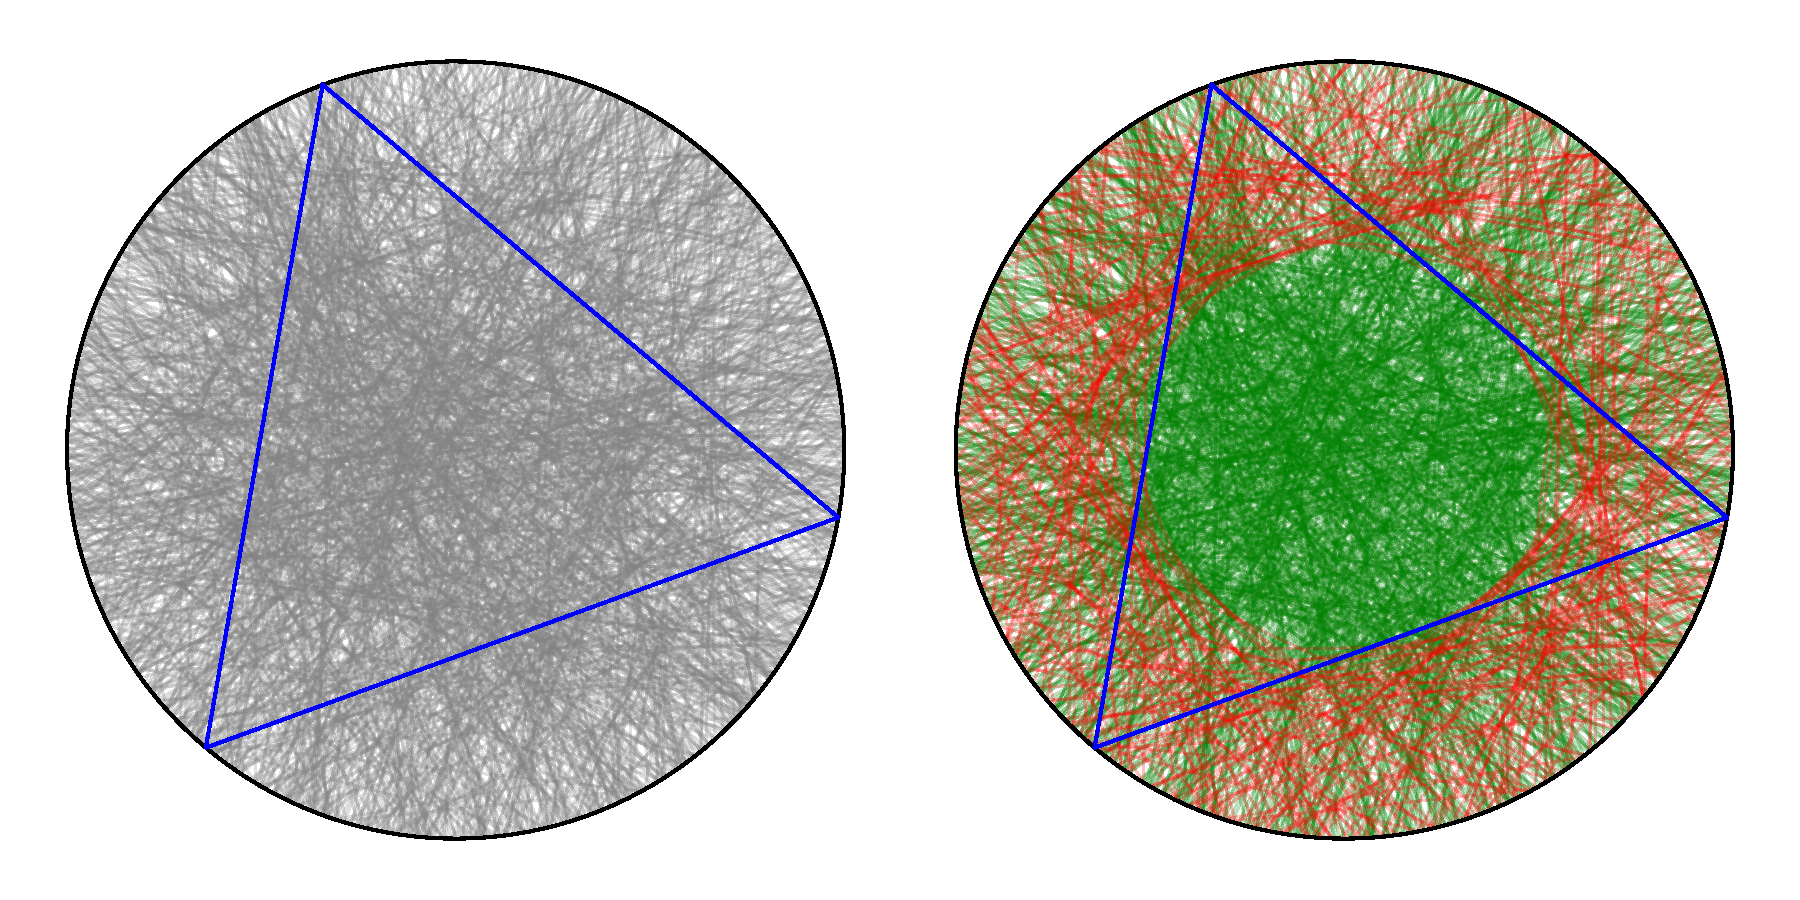
\includegraphics[width=\linewidth]{images/chords_distribution.pdf}
		\caption{Left: the $N = 1000$ random chords generated with the procedure of Figure~\ref{fig:definition}. Right: the same chords, in green if longer than the side of the inscribed triangle and in red otherwise.}
		\label{fig:distribution}
	\end{figure}
	\FloatBarrier
	
	\section*{Dependence of the estimate on the number of extractions}
	
	To study how the precision of the estimated probability improves with the number of extractions, the whole procedure is repeated for $N = 10^k$ chords, with $k = 2, \dots, 7$.
	For each value of $N$ an independent set of chords is generated, and the probability and its uncertainty are computed as in Eq.~\eqref{eq:sigma}.
	The results are reported in Table~\ref{tab:convergence}.
	
	\begin{table}[!h]
		\centering
		\begin{tabular}{c c c}
			\hline
			$N$ & $P$ & $\sigma_P$ \\
			\hline
			$10^2$ & $0.82000$ & $0.03842$ \\
			$10^3$ & $0.72800$ & $0.01407$ \\
			$10^4$ & $0.75080$ & $0.00433$ \\
			$10^5$ & $0.74746$ & $0.00137$ \\
			$10^6$ & $0.74680$ & $0.00043$ \\
			$10^7$ & $0.74701$ & $0.00014$ \\
			\hline
		\end{tabular}
		\caption{Estimate of the probability $P(L > \ell)$ and its statistical uncertainty for different numbers of extractions $N$.}
		\label{tab:convergence}
	\end{table}
	\FloatBarrier
	
	As $N$ grows, the estimate of $P$ stabilises and its uncertainty decreases.
	To quantify this behaviour, $\sigma_P$ is plotted as a function of $N$ in log-log scale (Figure~\ref{fig:convergence}) and fitted with the least-squares method (\texttt{scipy.optimize.curve\_fit}) with a straight line
	\begin{equation}
		\log_{10}\sigma_P = \alpha\, \log_{10} N + c \qquad \Longleftrightarrow \qquad \sigma_P \propto N^{\alpha}.
	\end{equation}
	The fit gives
	\begin{equation}
		\alpha_{fit} = -0.493 \pm 0.005,
	\end{equation}
	compatible with the expected value $\alpha = -1/2$.
	The statistical uncertainty therefore decreases as $1/\sqrt{N}$: to gain one more significant digit, the number of extractions has to be increased by a factor of 100.
	
	\begin{figure}[!h]
		\centering
		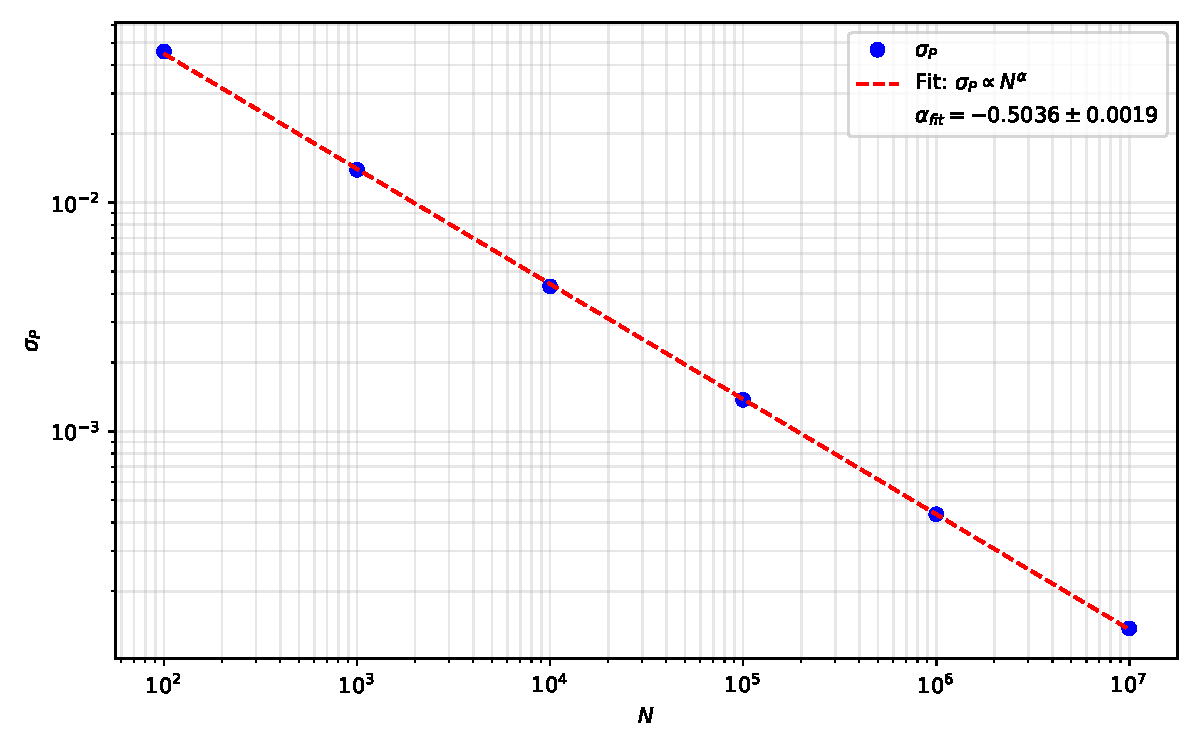
\includegraphics[width=0.95\linewidth]{images/convergence.pdf}
		\caption{Statistical uncertainty $\sigma_P$ as a function of the number of extractions $N$, in log-log scale. The dashed red line is the linear fit $\sigma_P \propto N^{\alpha}$.}
		\label{fig:convergence}
	\end{figure}
	\FloatBarrier
	
	\section*{Result}
	
	With the definition of random chord as the line through two points uniformly distributed inside the disk, the best estimate of the probability that a random chord is longer than the side of the inscribed equilateral triangle, obtained with $N = 10^7$ extractions, is
	\begin{equation}
		P = 0.74701 \pm 0.00014 .
	\end{equation}
	This value is different from all the three solutions presented in class ($1/3$, $1/2$, $1/4$), confirming that the answer to Bertrand's problem depends on the definition of random chord.
	
	
\end{document}
